\documentclass{beamer}
\usetheme{Berlin}
\setbeamertemplate{caption}[numbered]

\title{Systems with a Small Number of
Variables}
\subtitle{Course: Complex Systems Modeling}
\author{Robert Flassig}
\institute{Brandenburg University of Applied Sciences}
\date{\today}

\begin{document}
\begin{frame}
\titlepage
\end{frame}

\begin{frame}
\frametitle{Outline}
\tableofcontents
\end{frame}

\section{Linear Stability Analysis in 2 Dimensions}

\begin{frame}
  \frametitle{Recap: Linear Systems in One Dimension}
  \begin{itemize}
    \item 1D systems: \(\dot{x} = f(x)\)
    \item Stability determined by slope \(f'(x^*)\)
    \item Phase line: arrows show motion → fixed points divide regions
    \item For nonlinear \(f(x)\): graphical analysis suffices, but limited to 1D
  \end{itemize}
  \begin{block}{Motivation}
    Real systems (oscillators, populations, circuits) need \(\ge 2\) state variables.
  \end{block}
\end{frame}

\begin{frame}
  \frametitle{From 1D to 2D Systems}
  \[
  \dot{x} = a x + b y,\quad \dot{y} = c x + d y
  \]
  \begin{itemize}
    \item Four parameters \(a,b,c,d\) define linear coupling
    \item In vector form:
    \[
    \dot{\mathbf{x}} = A \mathbf{x}, \quad
    A = \begin{pmatrix} a & b \\ c & d \end{pmatrix}
    \]
    \item The origin \(\mathbf{x}^* = (0,0)\) is always a fixed point.
  \end{itemize}
  \begin{block}{Superposition Principle}
    If \(\mathbf{x}_1,\mathbf{x}_2\) are solutions, so is any \(c_1\mathbf{x}_1 + c_2\mathbf{x}_2\).
  \end{block}
\end{frame}

\begin{frame}
  \frametitle{The Phase Plane}
  \begin{itemize}
    \item The pair \((x,y)\) represents the \emph{state} of the system.
    \item Trajectories evolve in the $(x,y)$ plane $\rightarrow$ \emph{phase plane}.
    \item Each point has a velocity vector given by the ODE:
    \[
      \dot{\mathbf{x}} = A \mathbf{x}
    \]
    \item The resulting pattern of arrows is the \emph{vector field}.
  \end{itemize}
  \centering
  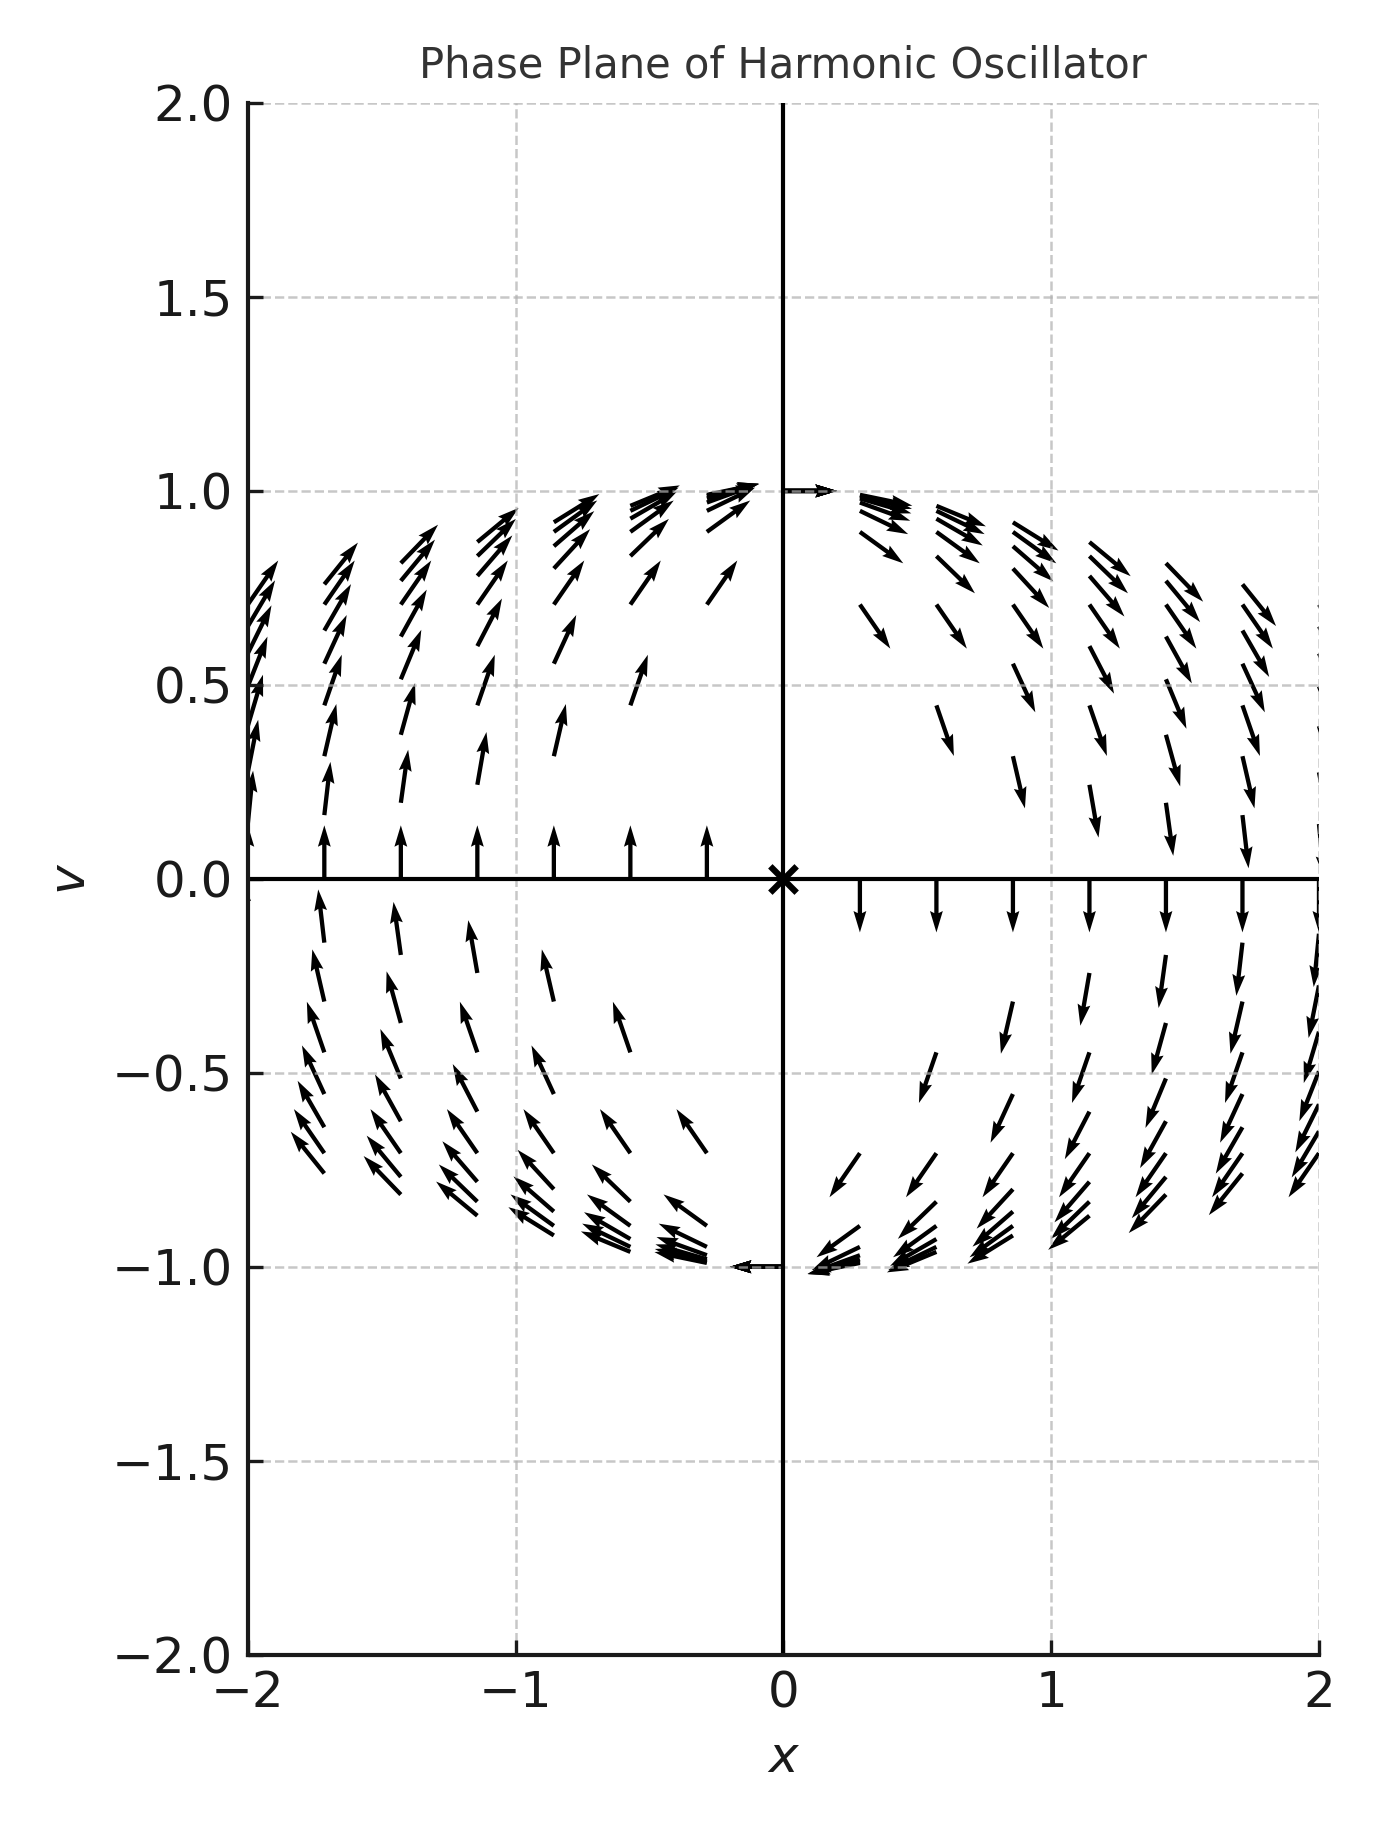
\includegraphics[width=0.3\textwidth]{phase_plane_schematic.png}
\end{frame}

%--------------------------------------------------------

\begin{frame}
  \frametitle{Example: The Linear Spring–Mass System}
  \[
  m \ddot{x} + kx = 0
  \]
  \begin{columns}[T]
    \begin{column}{0.55\textwidth}
      Let \(v = \dot{x}\), then:
      \[
      \dot{x} = v,\quad \dot{v} = -\frac{k}{m}x
      \]
      Define \(\omega_0^2 = \frac{k}{m}\):
      \[
      \dot{x} = v,\quad \dot{v} = -\omega_0^2 x
      \]
      $\Rightarrow$ state \((x,v)\) evolves on the phase plane.
    \end{column}
    \begin{column}{0.4\textwidth}
      \centering
      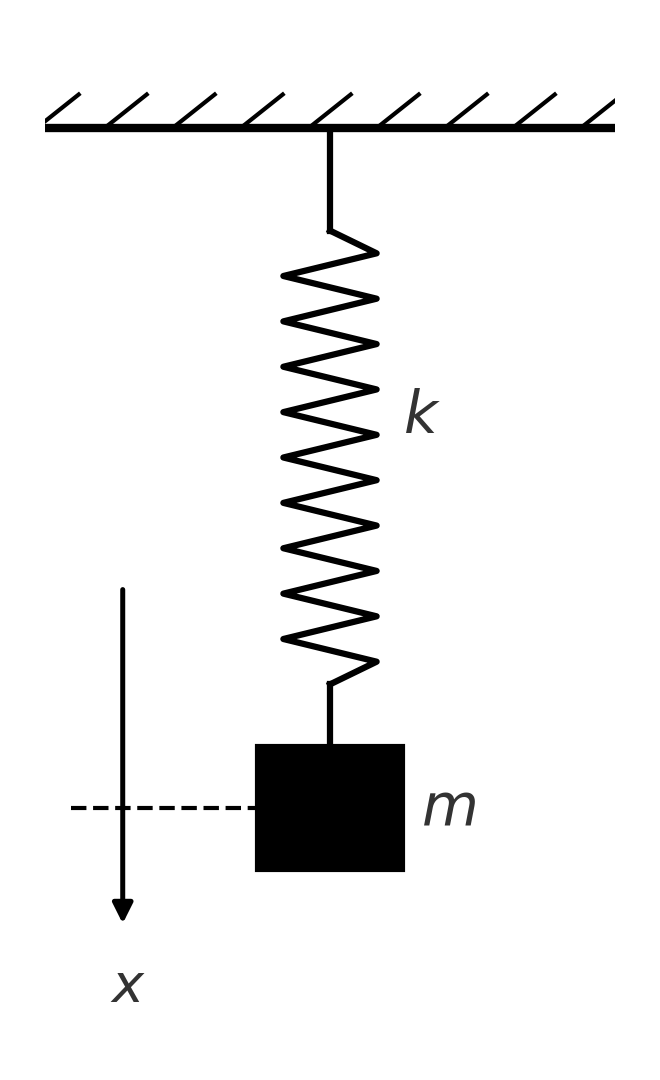
\includegraphics[width=0.45\textwidth]{spring_mass.png}
    \end{column}
  \end{columns}
\end{frame}

%--------------------------------------------------------

\begin{frame}
  \frametitle{Vector Field Interpretation}
  \begin{itemize}
    \item Each point \((x,v)\) has velocity:
      \[
      \mathbf{F}(x,v) = (\dot{x},\dot{v}) = (v, -\omega_0^2 x)
      \]
    \item On \(x\)-axis (\(v=0\)): vectors point vertically (\(\dot{v}=-\omega_0^2 x\))
    \item On \(v\)-axis (\(x=0\)): vectors point horizontally (\(\dot{x}=v\))
    \item Flow forms a circulating pattern about origin
  \end{itemize}
  \centering
  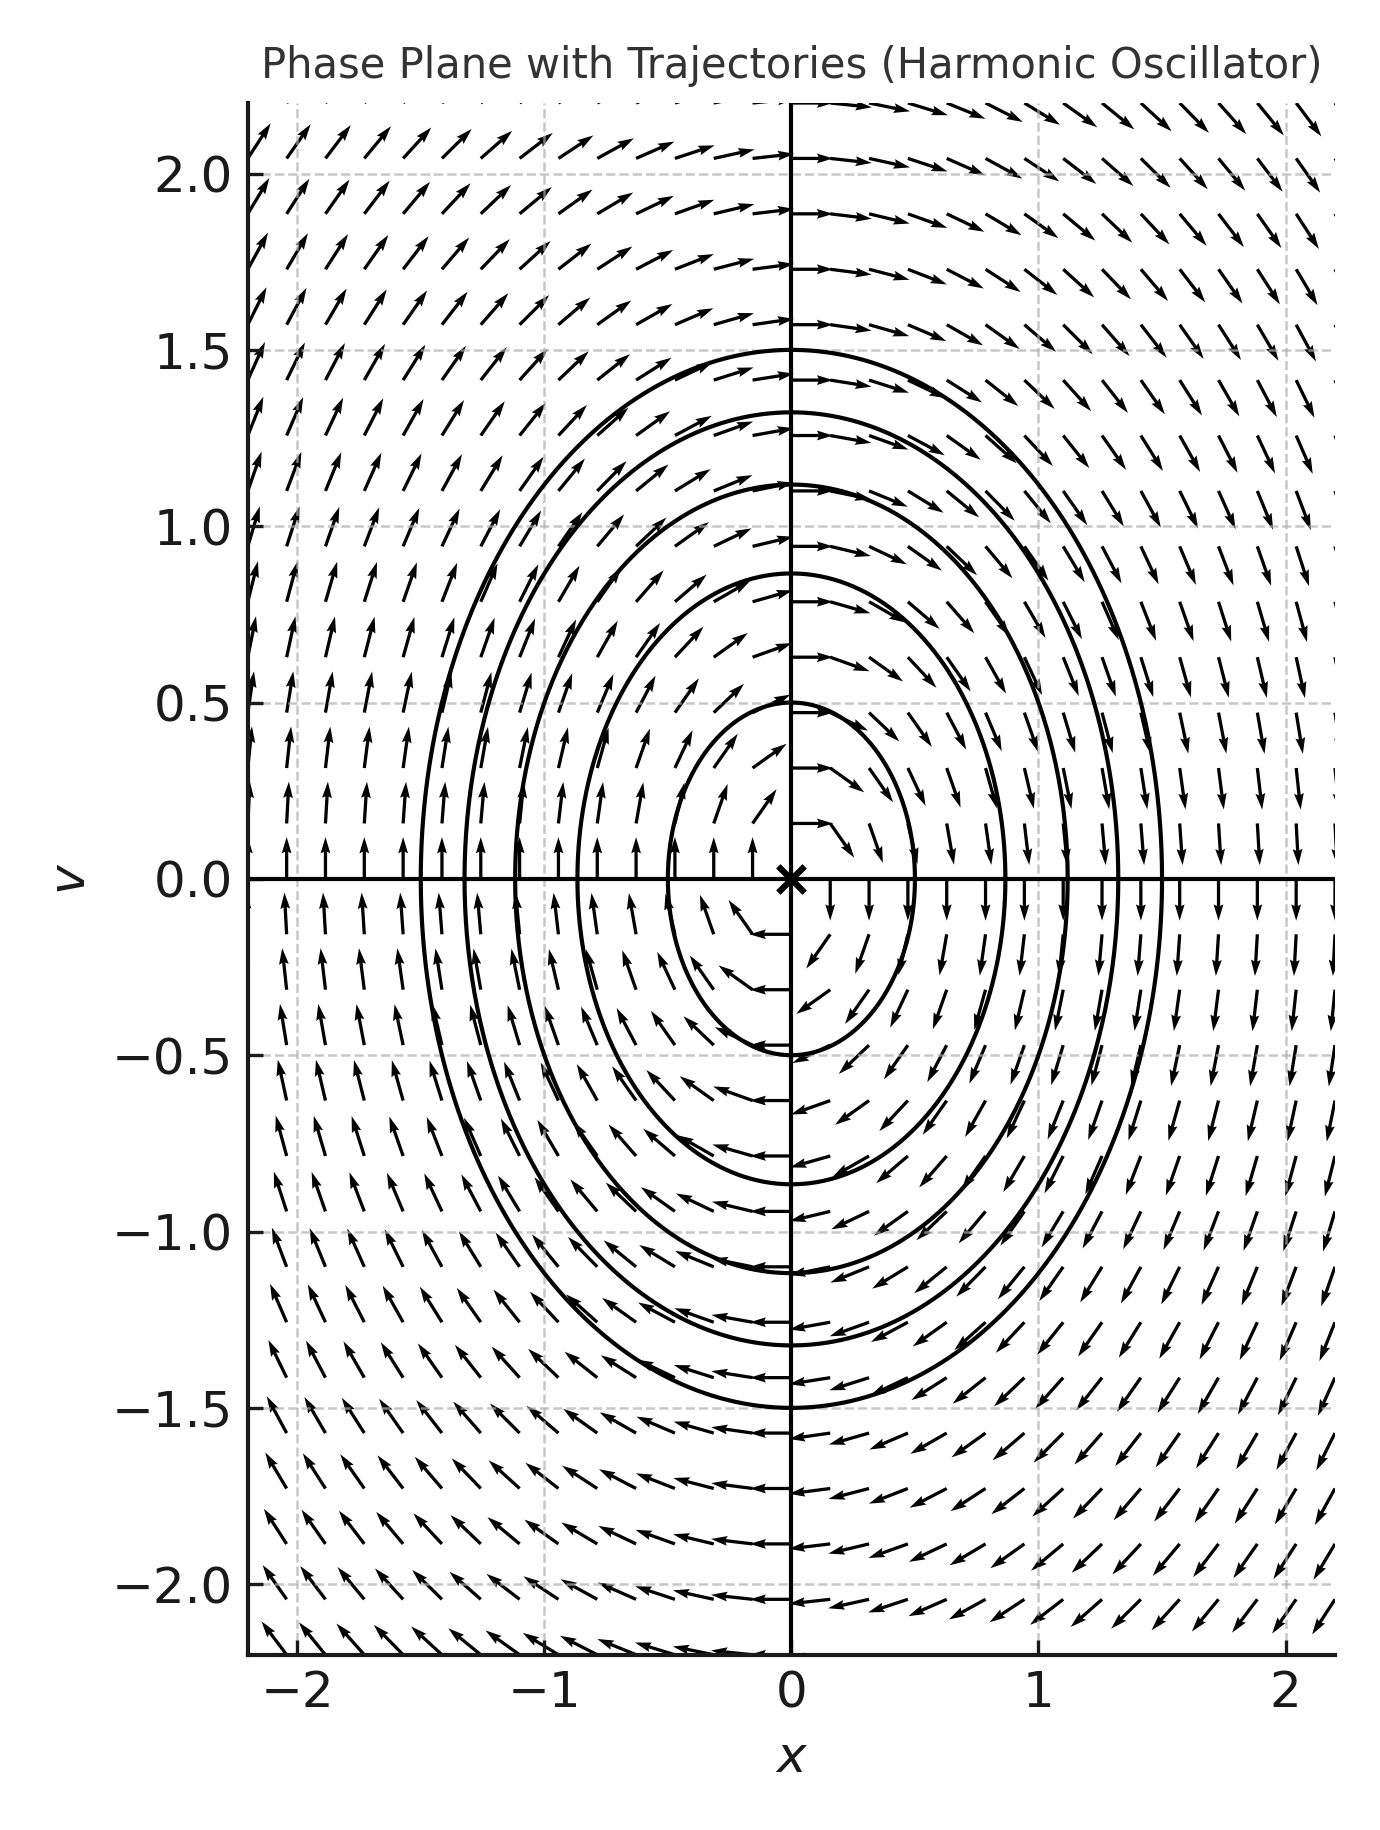
\includegraphics[width=0.3\textwidth]{phase_vector_field.png}
\end{frame}

%--------------------------------------------------------

\begin{frame}
  \frametitle{Phase Portrait of the Harmonic Oscillator}
  \begin{itemize}
    \item The origin \((0,0)\) is a \emph{fixed point} (equilibrium).
    \item All other trajectories form \emph{closed orbits} (periodic motion).
    \item Energy is conserved: \(E = \tfrac{1}{2}m v^2 + \tfrac{1}{2}k x^2 = \text{const.}\)
    \item Hence, orbits satisfy \(v^2 + \omega_0^2 x^2 = C\) $\rightarrow$ \emph{ellipses}.
  \end{itemize}
  \centering
  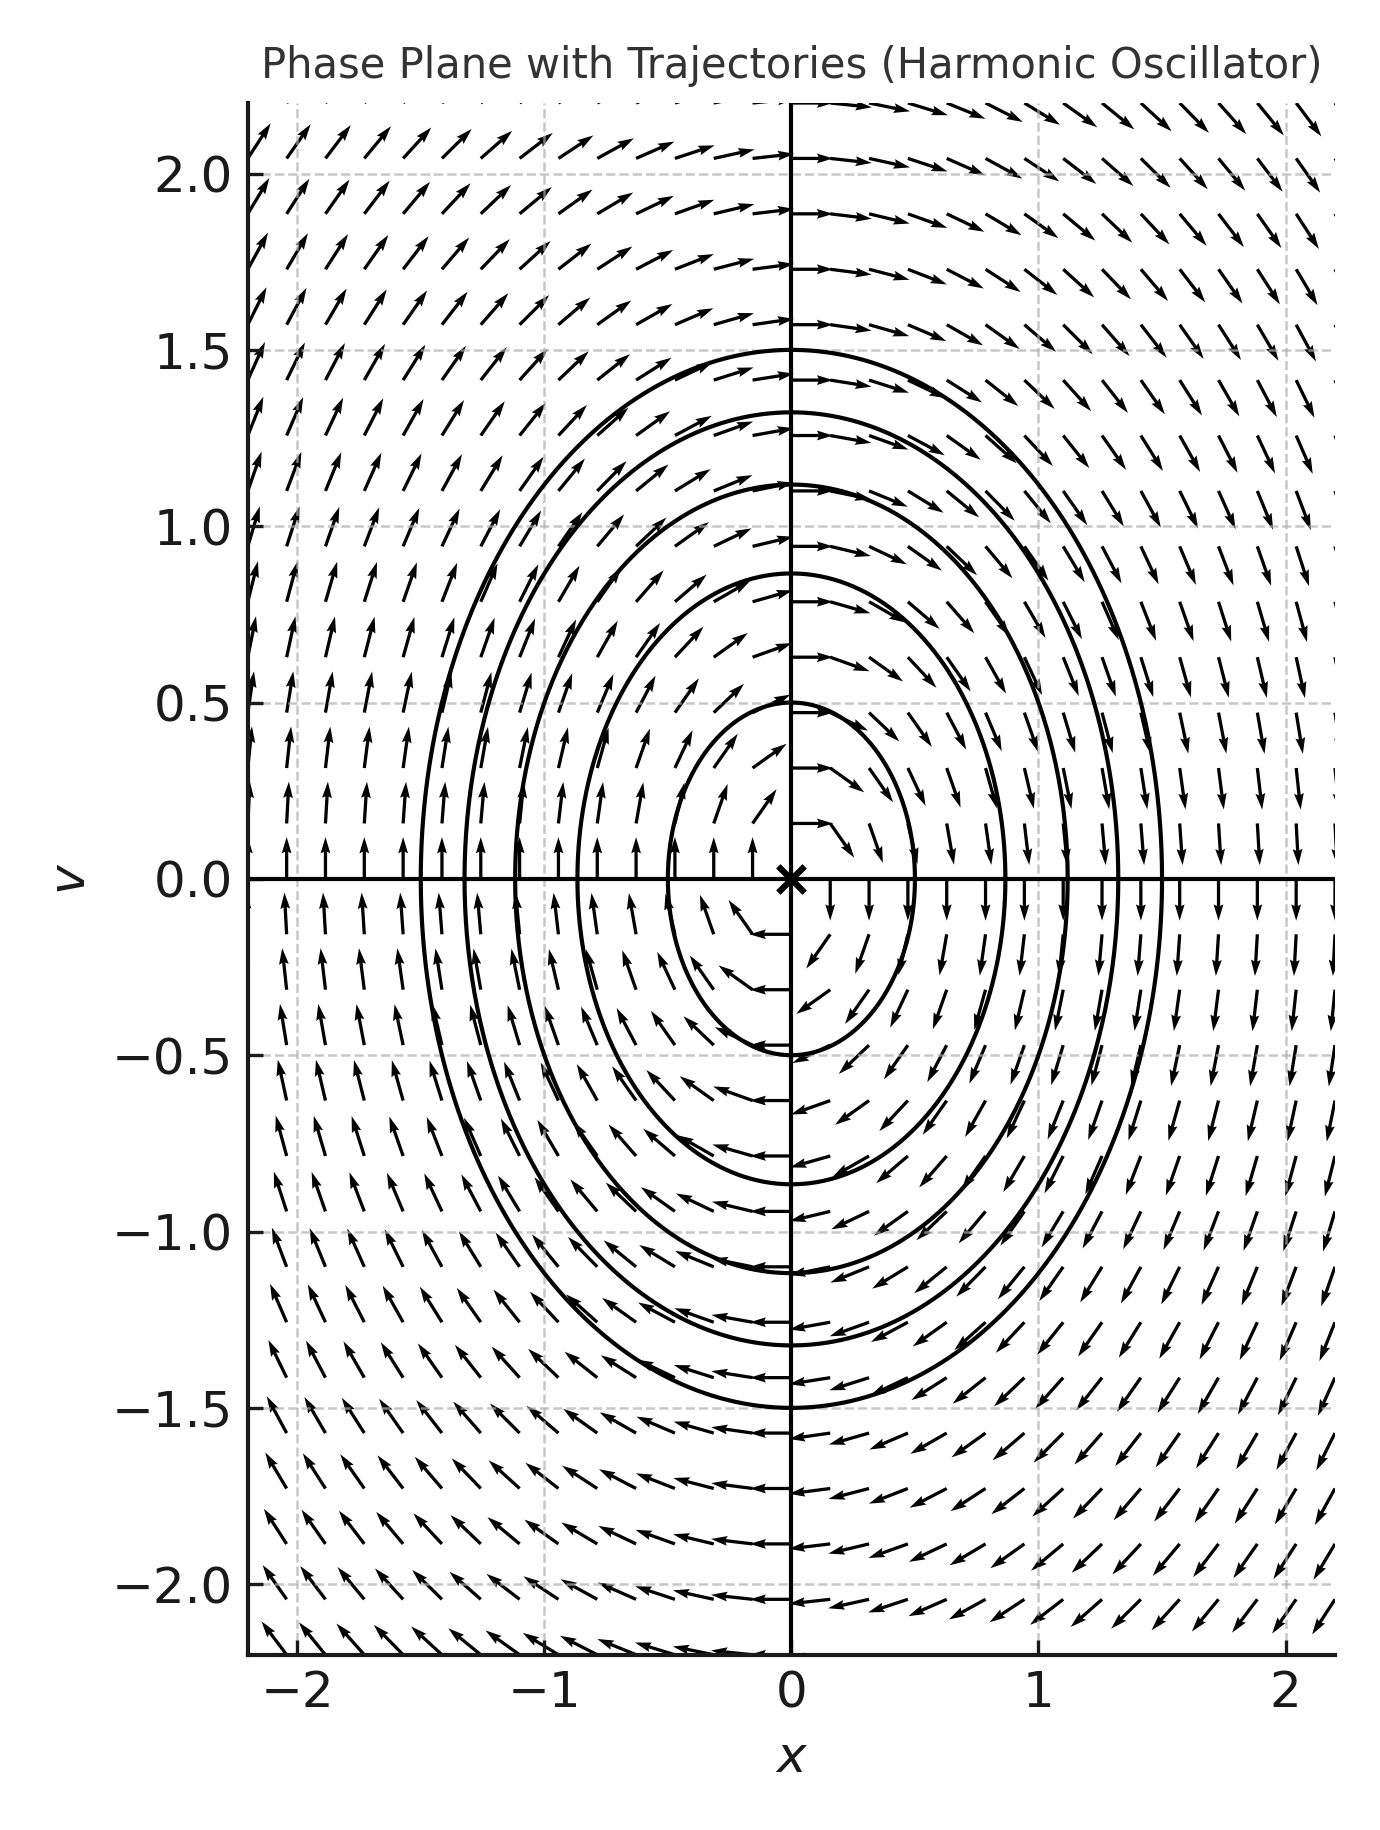
\includegraphics[width=0.35\textwidth]{phase_vector_field.png}
\end{frame}

%--------------------------------------------------------

\begin{frame}
  \frametitle{Physical Interpretation}
  \begin{columns}[T]
    \begin{column}{0.6\textwidth}
      \begin{itemize}
        \item Fixed point = static equilibrium (mass at rest)
        \item Closed orbit = periodic motion (oscillation)
        \item Direction along orbit shows time evolution:
          \begin{align*}
            x<0, v=0 &\Rightarrow \text{max compression} (a) \\
            x=0, v>0 &\Rightarrow \text{passes equilibrium}  (b)\\
            x>0, v=0 &\Rightarrow \text{max extension} (c)
          \end{align*}
      \end{itemize}
    \end{column}
    \begin{column}{0.4\textwidth}
      \begin{figure}
        \centering
        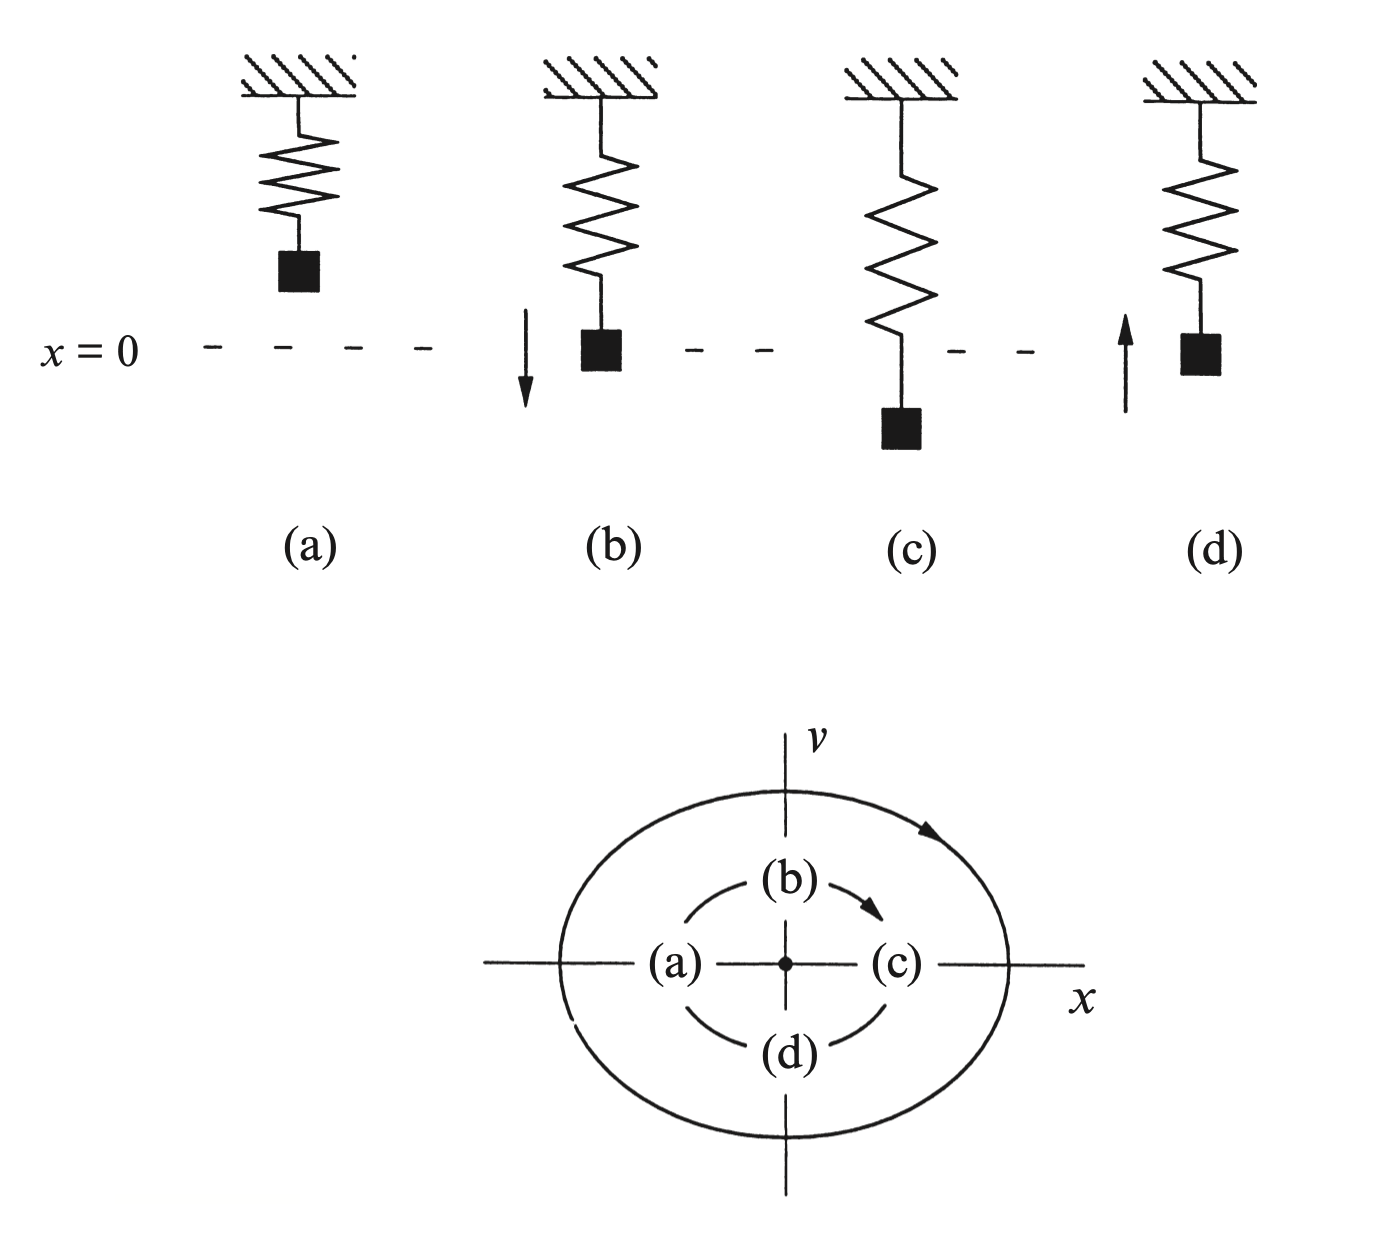
\includegraphics[width=\textwidth]{oscillator_cycle.png}
        \caption{\scriptsize Harmonic oscillator phase portrait with labeled cycle points.}
      \end{figure}
    \end{column}
  \end{columns}
\end{frame}


%--------------------------------------------------------


\begin{frame}
  \frametitle{Example: System and Setup}
  \vspace{-0.2em}
  \[
    \dot{\mathbf{x}} = A\,\mathbf{x},\quad
    A=\begin{pmatrix} a & 0 \\ 0 & -1 \end{pmatrix},\qquad
    \mathbf{x}=\begin{pmatrix}x\\y\end{pmatrix}
  \]
  \begin{itemize}
    \item Uncoupled ODEs: \(\dot{x}=a\,x,\quad \dot{y}=-\,y\).
    \item Fixed points: always \(\mathbf{x}^*=(0,0)\); special case \(a=0\) gives a whole line \(\{(x,0)\}\).
    \item Solution with initial \((x_0,y_0)\):
      \[
        x(t)=x_0\,e^{a t},\qquad y(t)=y_0\,e^{-t}.
      \]
  \end{itemize}
  \begin{block}{Trajectory slope (useful for portrait)}
  \small
    \(\displaystyle \frac{dy}{dx}=\frac{\dot y}{\dot x}=\frac{-y}{a\,x}\quad\Rightarrow\quad
      \ln|y|=-\frac{1}{a}\ln|x|+C\ \Rightarrow\ y=C\,x^{-1/a}\quad (a\neq 0).\)
  \end{block}
\end{frame}

%----------------------------------------


\begin{frame}
  \frametitle{Phase Portraits for Different Values of $a$}
  \begin{itemize}
    \item Each panel shows the phase portrait of
      \[
        \dot{x}=a x,\quad \dot{y}=-y
      \]
      as the parameter \(a\) varies.
    \item The qualitative behavior changes at
      \(a=-1,\,0\).
  \end{itemize}
  \vspace{0.4em}
  \begin{figure}
    \centering
    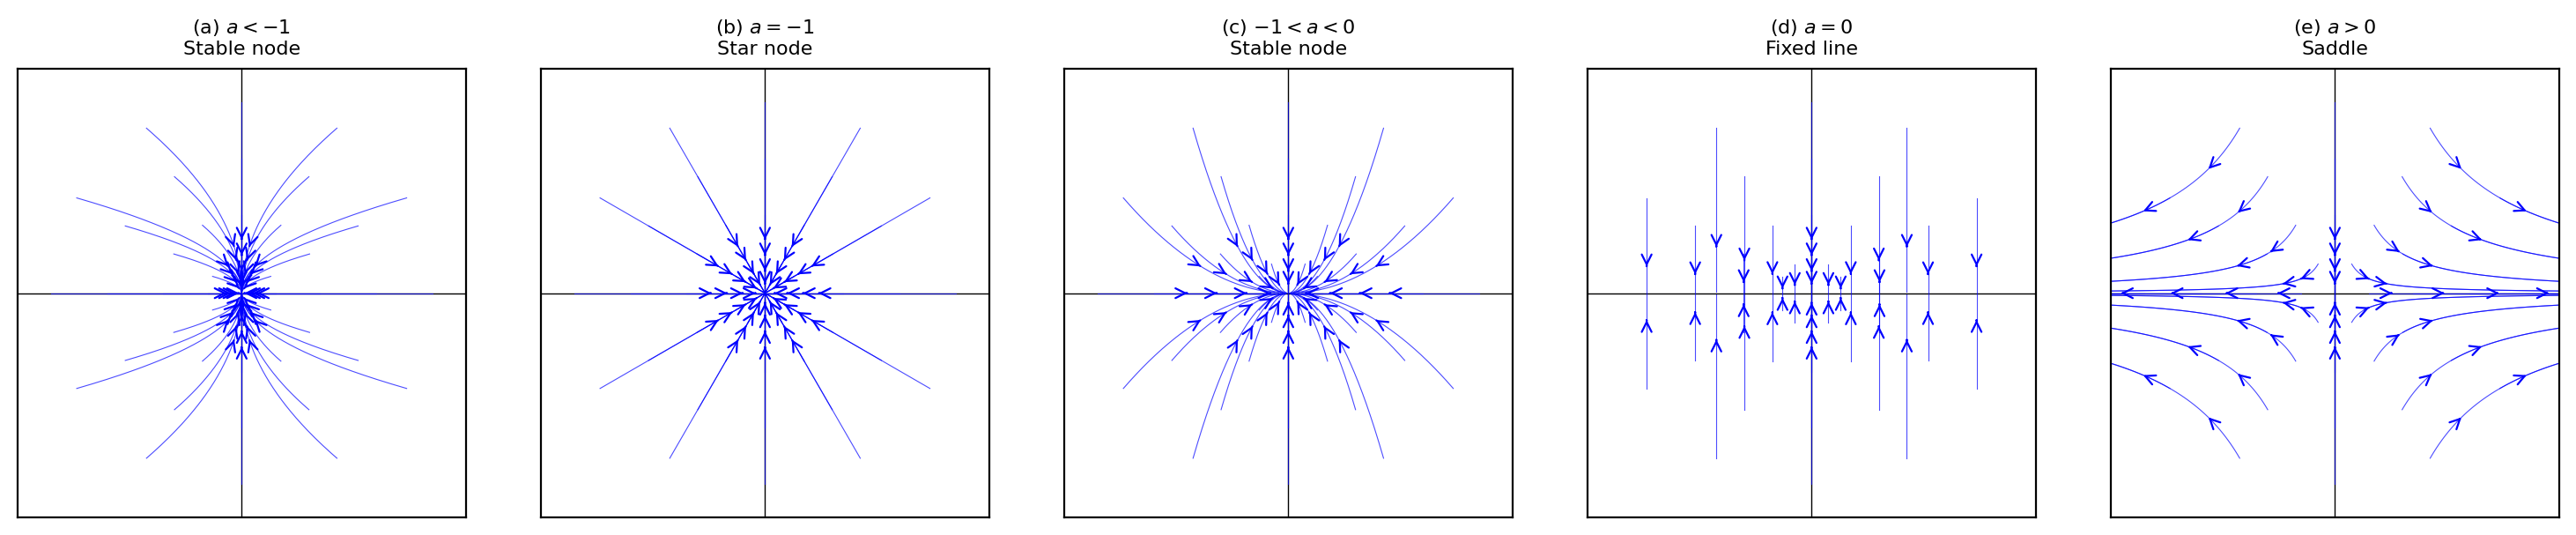
\includegraphics[width=0.85\textwidth]{phase_portraits_nodes.png}
    \caption{\tiny Phase portraits for different values of $a$.}
    \label{fig:phase_portraits_nodes}
  \end{figure}
\end{frame}


\begin{frame}
  \frametitle{Case I: $a<-1$ (Stable node; approach tangential to $y$-axis)}
  \begin{itemize}
    \item Both \(x(t)\) and \(y(t)\) decay \(\Rightarrow\) stable fixed point at the origin.
    \item \( |a|>1 \Rightarrow\) \(x(t)\) decays \emph{faster} than \(y(t)\).
    \item Forward time: trajectories approach tangent to the \textbf{slower} direction (the \(y\)-axis).
    \item Backward time: become parallel to the \textbf{faster} direction (the \(x\)-axis).
  \end{itemize}
\end{frame}

%----------------------------------------

\begin{frame}
  \frametitle{Case II: $a=-1$ (Star/symmetric node)}
  \begin{itemize}
    \item Equal decay rates in \(x\) and \(y\).
    \item From solutions: \(\displaystyle \frac{y(t)}{x(t)}=\frac{y_0}{x_0}\) is constant.
    \item \(\Rightarrow\) All trajectories are straight lines through the origin.
    \item This degenerate, measure-zero case is the \textbf{star} (or symmetric) node.
  \end{itemize}
\end{frame}

%----------------------------------------

\begin{frame}
  \frametitle{Case III: $-1<a<0$ (Stable node; approach tangential to $x$-axis)}
  \begin{itemize}
    \item Still stable: \(x(t)\to 0\), \(y(t)\to 0\).
    \item Now \(|a|<1 \Rightarrow\) \(x(t)\) decays \emph{slower} than \(y(t)\).
    \item Trajectories approach tangent to the \textbf{slower} direction (the \(x\)-axis).
  \end{itemize}
\end{frame}

%----------------------------------------

\begin{frame}
  \frametitle{Case IV: $a=0$ (Line of fixed points)}
  \begin{itemize}
    \item \(\dot x = 0 \Rightarrow x(t)\equiv x_0\) (constant); \(\ \dot y=-y\Rightarrow y(t)\to 0.\)
    \item Every point on the \(\{(x,0)\}\) line is an equilibrium.
    \item Trajectories are vertical lines \(x(t)=x_0\) approaching the \(x\)-axis.
  \end{itemize}
\end{frame}

%----------------------------------------

\begin{frame}
  \frametitle{Case V: $a>0$ (Saddle)}
  \begin{itemize}
    \item \(x(t)=x_0 e^{a t}\) grows; \(y(t)=y_0 e^{-t}\) decays.
    \item \(\Rightarrow\) The origin is an \textbf{unstable} fixed point (saddle).
    \item Stable manifold: \(y\)-axis \((x_0=0)\) $\Rightarrow$ \(x(t)\equiv 0,\ y(t)\to 0\).
    \item Unstable manifold: \(x\)-axis \((y_0=0)\) $\Rightarrow$ \(y(t)\equiv 0,\ x(t)\to \pm\infty\).
    \item Typical trajectories: asymptotic to the unstable manifold in forward time, to the stable manifold in backward time.
  \end{itemize}
\end{frame}

%----------------------------------------

\begin{frame}
  \frametitle{Summary: Classification vs.\ Parameter $a$}
  \vspace{-0.3em}
  \begin{columns}[T]
    \begin{column}{0.6\textwidth}
      \begin{itemize}
        \item \(\lambda_1=a,\ \lambda_2=-1\) (eigenvalues of \(A\)).
        \item \(\;\;a<-1:\) stable node, approach tangent to \(y\)-axis.
        \item \(\;\;a=-1:\) star/symmetric node (straight lines).
        \item \(-1<a<0:\) stable node, approach tangent to \(x\)-axis.
        \item \(\;\;a=0:\) line of equilibria (\(x\)-axis).
        \item \(\;\;a>0:\) saddle; \(W^s=\{x=0\},\ W^u=\{y=0\}\).
      \end{itemize}
    \end{column}
    \begin{column}{0.4\textwidth}
      \begin{block}{Invariant curves (for $a\neq 0$)}
        \(y = C\,x^{-1/a}\) \\
        (level sets that trajectories follow)
      \end{block}
    \end{column}
  \end{columns}
\end{frame}

%========================================================
\section{Stability Language}
%========================================================

\begin{frame}
  \frametitle{Stability Language}
  \tiny
  \begin{itemize}
    \item To describe how trajectories behave near fixed points, we introduce key stability terms.
    \item These notions apply to both linear and nonlinear systems.
  \end{itemize}

  \vspace{0.4em}
  \begin{block}{Attracting Fixed Point}
    \begin{itemize}
      \item \( \mathbf{x}^* \) is \textbf{attracting} if trajectories starting near it satisfy
        \[
          \mathbf{x}(t) \to \mathbf{x}^* \quad \text{as } t \to \infty.
        \]
      \item In Figs. \ref{fig:phase_portraits_nodes} (a–c): the origin attracts all trajectories (globally attracting).
    \end{itemize}
  \end{block}

  \begin{block}{Liapunov Stability}
    \begin{itemize}
      \item \( \mathbf{x}^* \) is \textbf{Liapunov stable} if trajectories that start close stay close for all \(t>0\).
      \item Figs.  \ref{fig:phase_portraits_nodes} (a–d): origin is Liapunov stable.
    \end{itemize}
  \end{block}
\end{frame}

%--------------------------------------------------------

\begin{frame}
  \frametitle{Types of Stability}
  \tiny
  \begin{columns}[T]
    \begin{column}{0.58\textwidth}
      \begin{itemize}
        \item \textbf{Neutrally stable:} Liapunov stable but not attracting.\\
          – Nearby trajectories neither converge nor diverge.\\
          – Example: harmonic oscillator (\(\dot{x}=v,\; \dot{v}=-x\)).
        \item \textbf{Asymptotically stable:} both Liapunov stable and attracting.
        \item \textbf{Unstable:} neither attracting nor Liapunov stable.
      \end{itemize}
      \vspace{0.5em}
      \begin{block}{Notation}
        Solid black dot   →  Liapunov stable \\
        Open dot   →  Unstable
      \end{block}
    \end{column}
    \begin{column}{0.42\textwidth}
      \centering
      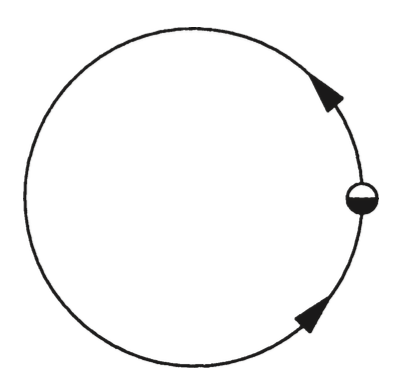
\includegraphics[width=\textwidth]{stability_language.png}\\[2pt]
      {\scriptsize Types of stability for fixed points.}
    \end{column}
  \end{columns}
\end{frame}

%========================================================
\section{Classification of Linear Systems}
%========================================================

%--------------------------------------------------------
\begin{frame}
  \frametitle{Motivation: Beyond Special Matrices}
  \begin{itemize}
    \item Previously: special case with zeros in $A$ (easy to separate variables).
    \item Now: general $2\times2$ linear system
      \[
        \dot{\mathbf{x}} = A\mathbf{x}, \quad
        A=\begin{pmatrix} a & b \\ c & d \end{pmatrix}.
      \]
    \item Goal: classify all possible phase portraits by properties of $A$.
    \item Idea: find \emph{special trajectories} analogous to the coordinate axes.
  \end{itemize}
\end{frame}

%--------------------------------------------------------
\begin{frame}
  \frametitle{Searching for Straight-Line Trajectories}
  \begin{itemize}
    \item Assume motion along a fixed direction $\mathbf{v}$ with exponential time dependence:
      \[
        \mathbf{x}(t) = e^{\lambda t}\mathbf{v}, \quad \mathbf{v}\neq 0.
      \]
    \item Substitute into $\dot{\mathbf{x}}=A\mathbf{x}$:
      \[
        \lambda e^{\lambda t}\mathbf{v} = e^{\lambda t}A\mathbf{v}
        \ \Rightarrow\ (A-\lambda I)\mathbf{v}=0.
      \]
    \item Nontrivial solutions exist $\iff$ $\mathbf{v}$ is an \textbf{eigenvector} of $A$
      with eigenvalue $\lambda$.
    \item Then $\mathbf{x}(t)=e^{\lambda t}\mathbf{v}$ is called an \textbf{eigensolution}.
  \end{itemize}
\end{frame}

%--------------------------------------------------------
\begin{frame}
  \frametitle{Eigenvalues and Eigenvectors of a $2\times2$ Matrix}
  \begin{columns}[T]
    \begin{column}{0.52\textwidth}
      \begin{itemize}
        \item Characteristic equation:
          \[
            \det(A-\lambda I)=0.
          \]
        \item For
          \(
            A=\begin{pmatrix} a & b \\ c & d \end{pmatrix}
          \),
          expansion gives
          \[
            \lambda^2 - (a+d)\lambda + (ad-bc)=0.
          \]
        \item Define:
          \[
            \tau=\mathrm{tr}(A)=a+d,\quad
            \Delta=\det(A)=ad-bc.
          \]
      \end{itemize}
    \end{column}
    \begin{column}{0.48\textwidth}
      \begin{block}{Eigenvalues}
        \[
        \lambda_{1,2} = \frac{\tau \pm \sqrt{\tau^2-4\Delta}}{2}.
        \]
      \end{block}
      \vspace{0.3em}
      \begin{block}{Eigenvectors}
        $(A-\lambda_i I)\mathbf{v}_i=0$
      \end{block}
    \end{column}
  \end{columns}
\end{frame}

%--------------------------------------------------------
\begin{frame}
  \frametitle{General Solution for Distinct Eigenvalues}
  \begin{itemize}
    \item If $\lambda_1\neq\lambda_2$, the eigenvectors $\mathbf{v}_1,\mathbf{v}_2$ are linearly independent.
    \item Any initial condition can be written as
      \[
        \mathbf{x}_0=c_1\mathbf{v}_1+c_2\mathbf{v}_2.
      \]
    \item Hence the general solution is
      \[
        \mathbf{x}(t)=c_1 e^{\lambda_1 t}\mathbf{v}_1 + c_2 e^{\lambda_2 t}\mathbf{v}_2.
      \]
    \item The coefficients $c_1,c_2$ follow from $\mathbf{x}(0)=\mathbf{x}_0$.
  \end{itemize}
  \vspace{0.4em}
  \begin{block}{Interpretation}
    Each eigendirection defines a straight-line trajectory with exponential growth or decay rate $\lambda_i$.
  \end{block}
\end{frame}

\begin{frame}
  \frametitle{Geometric Interpretation of the Solution}
  \small
  \begin{itemize}
    \item Any initial condition \(\mathbf{x}_0\) can be expressed as a linear combination
      of eigenvectors:
      \[
        \mathbf{x}_0 = c_1\mathbf{v}_1 + c_2\mathbf{v}_2.
      \]
    \item Each component evolves independently along its eigendirection:
      \[
        \mathbf{x}(t) = c_1 e^{\lambda_1 t}\mathbf{v}_1 + c_2 e^{\lambda_2 t}\mathbf{v}_2.
      \]
    \item The phase portrait is obtained by superimposing these exponential motions.
    \item The relative magnitudes of \(e^{\lambda_1 t}\) and \(e^{\lambda_2 t}\) determine the trajectory’s shape.
  \end{itemize}
  \vspace{0.6em}
  \centering
  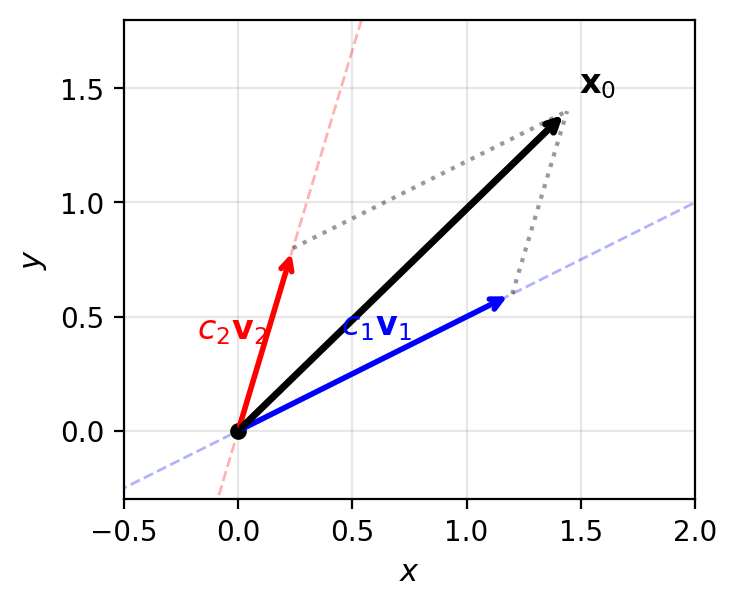
\includegraphics[width=0.15\textwidth]{eigen_decomposition.png}\\[2pt]
  {\scriptsize Decomposition of an initial condition into eigenvector components.}
\end{frame}


%--------------------------------------------------------
\begin{frame}
  \frametitle{Example: Solving a Specific System}
  \[
    \dot{x}=x+y, \qquad
    \dot{y}=-4x-2y,
  \]
  with initial condition $(x_0,y_0)=(2,3)$.
  \begin{itemize}
    \item Matrix form:
      \(
        A=\begin{pmatrix} 1 & 1 \\ -4 & -2 \end{pmatrix}.
      \)
    \item Characteristic equation:
      \(
        \lambda^2 + \lambda - 6 = 0 \Rightarrow
        \lambda_1=2,\; \lambda_2=-3.
      \)
    \item Eigenvectors:
      \[
        \lambda_1=2\Rightarrow \mathbf{v}_1=\begin{pmatrix}1\\-1\end{pmatrix},\quad
        \lambda_2=-3\Rightarrow \mathbf{v}_2=\begin{pmatrix}1\\4\end{pmatrix}.
      \]
  \end{itemize}
\end{frame}

%--------------------------------------------------------
\begin{frame}
  \frametitle{Example (cont’d): General and Particular Solution}
  \begin{itemize}
    \item \textbf{General solution:}
      \[
        \mathbf{x}(t)
        = c_1 e^{2t}
          \begin{pmatrix}1\\[-2pt]-1\end{pmatrix}
        + c_2 e^{-3t}
          \begin{pmatrix}1\\[-2pt]4\end{pmatrix}.
      \]
    \item Apply the initial condition $(x_0,y_0)=(2,3)$:
      \[
        \begin{cases}
          2 = c_1 + c_2,\\[3pt]
          3 = -c_1 + 4c_2,
        \end{cases}
        \qquad \Rightarrow \quad c_1 = 1,\; c_2 = 1.
      \]
    \item Hence the \textbf{particular solution} is
      \[
        x(t)=e^{2t}+e^{-3t}, \qquad
        y(t)=-\,e^{2t}+4e^{-3t}.
      \]
    \item Interpretation:
      \begin{itemize}
        \item Growth along eigenvector $\mathbf{v}_1=(1,-1)^\mathsf{T}$ with rate $\lambda_1=2$,
        \item Decay along eigenvector $\mathbf{v}_2=(1,4)^\mathsf{T}$ with rate $\lambda_2=-3$.
      \end{itemize}
  \end{itemize}
\end{frame}


%--------------------------------------------------------
\begin{frame}
  \frametitle{Example (cont’d): Phase Portrait and Manifolds}

  \begin{itemize}
    \item We found eigenvalues $\lambda_1=2$, $\lambda_2=-3$.
    \item One eigendirection grows, the other decays:
      \begin{itemize}
        \item $\lambda_1=2>0$: along $\mathbf{v}_1=(1,-1)^\mathsf{T}$
          solutions grow exponentially $\sim e^{2t}$.
        \item $\lambda_2=-3<0$: along $\mathbf{v}_2=(1,4)^\mathsf{T}$
          solutions decay exponentially $\sim e^{-3t}$.
      \end{itemize}
    \item Therefore, the origin is a \textbf{saddle point}.
      \begin{itemize}
        \item The \textbf{stable manifold} is the line
          spanned by $\mathbf{v}_2=(1,4)^\mathsf{T}$.
        \item The \textbf{unstable manifold} is the line
          spanned by $\mathbf{v}_1=(1,-1)^\mathsf{T}$.
      \end{itemize}
    \item A typical trajectory:
      \begin{itemize}
        \item approaches the stable manifold as $t\to -\infty$,
        \item and the unstable manifold as $t\to +\infty$.
      \end{itemize}
  \end{itemize}
\end{frame}

%--------------------------------------------------------
\begin{frame}
  \frametitle{Phase Portraits: Stable and Unstable Nodes}

  \begin{itemize}
    \item Consider a linear system $\dot{\mathbf{x}} = A\mathbf{x}$ with
      two \textbf{real, distinct} eigenvalues $\lambda_1,\lambda_2$ and
      eigenvectors $\mathbf{v}_1,\mathbf{v}_2$.
    \item \textbf{Stable node:} $\lambda_1<0$ and $\lambda_2<0$.
      \begin{itemize}
        \item Both eigensolutions decay exponentially.
        \item The origin is a \textbf{stable node}.
        \item Trajectories approach the origin \textbf{tangent to the slow
          eigendirection}, i.e.\ the eigenvector with smaller $|\lambda|$.
      \end{itemize}
    \item \textbf{Unstable node:} $\lambda_1>0$ and $\lambda_2>0$.
      \begin{itemize}
        \item Both eigensolutions grow exponentially.
        \item The origin is an \textbf{unstable node}.
        \item If we reverse all arrows in a stable-node phase portrait,
          we obtain a typical phase portrait for an unstable node.
      \end{itemize}
  \end{itemize}
\end{frame}

%--------------------------------------------------------
\begin{frame}
  \frametitle{Phase Portraits: Complex Eigenvalues}

  \begin{itemize}
    \item Eigenvalues:
      \[
        \lambda_{1,2}
        = \frac{\tau}{2} \pm \sqrt{\Bigl(\frac{\tau}{2}\Bigr)^2 - \Delta},
        \qquad \tau=\operatorname{tr}A,\; \Delta=\det A.
      \]
    \item Complex case: $(\tfrac{\tau}{2})^2 - \Delta < 0$
      \[
        \lambda_{1,2} = \alpha \pm i\omega,\quad \omega\neq 0.
      \]

    \item \textbf{Center} ($\alpha=0$):
      \begin{itemize}
        \item Purely imaginary eigenvalues.
        \item Closed orbits; fixed point is neutrally stable.
      \end{itemize}

    \item \textbf{Spiral / focus} ($\alpha\neq 0$):
      \begin{itemize}
        \item $\alpha<0$: stable spiral (damped oscillations).
        \item $\alpha>0$: unstable spiral (growing oscillations).
      \end{itemize}

    \item Rotation direction determined by checking the vector field.
  \end{itemize}
\end{frame}


%--------------------------------------------------------
\begin{frame}
  \frametitle{Phase Portraits: Repeated Eigenvalues}

  \begin{itemize}
    \item Repeated eigenvalue: $\lambda_1=\lambda_2=\lambda$.
    
    \item \textbf{Case 1: two independent eigenvectors}
      \begin{itemize}
        \item Eigenspace is 2D $\Rightarrow A=\lambda I$.
        \item $\lambda<0$: straight lines \emph{into} origin (stable star node).
        \item $\lambda>0$: straight lines \emph{out of} origin (unstable star node).
        \item $\lambda=0$: every point is fixed ($\dot{\mathbf{x}}=0$).
      \end{itemize}

    \item \textbf{Case 2: one eigenvector}
      \begin{itemize}
        \item Eigenspace is 1D $\Rightarrow$ \textbf{degenerate node}.
        \item Trajectories align with the single eigendirection as $t\to\pm\infty$.
        \item Lies on the boundary between a node and a spiral.
      \end{itemize}
  \end{itemize}

\end{frame}




%--------------------------------------------------------
\section{Trace–Determinant Classification}
%-----------
\begin{frame}
  \frametitle{Trace–Determinant Classification for $\dot{x}=Ax$}
  \begin{columns}[T]
    \begin{column}{0.52\textwidth}
      \begin{itemize}
      \item  \(
            A=\begin{pmatrix} a & b \\ c & d \end{pmatrix}
          \),
        \item Trace: \(\tau = a+d\), \quad Determinant: \(\Delta = ad - bc\).
        \item Eigenvalues:
          \[
            \lambda_{1,2}
            = \frac{\tau}{2}
              \pm \sqrt{\Bigl(\frac{\tau}{2}\Bigr)^2 - \Delta }.
          \]
        \item Discriminant: \(D=\tau^2-4\Delta.\)
        \item \(\Rightarrow\) Regions in the \((\tau,\Delta)\)-plane give:
          nodes, saddles, spirals, centers.
      \end{itemize}
    \end{column}
    \begin{column}{0.48\textwidth}
      \centering
      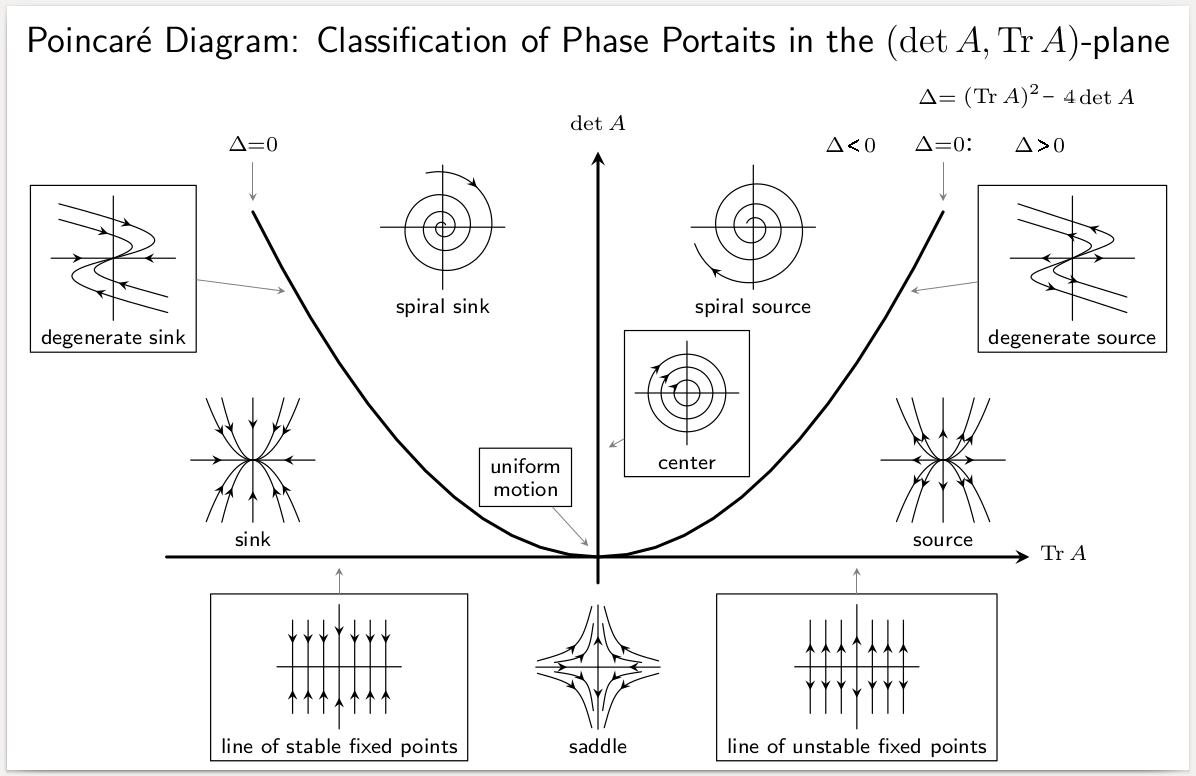
\includegraphics[width=\textwidth]{Stability_Diagram-2.png}\\[2pt]
      {\scriptsize Trace--determinant diagram. Credit: Freesodas, Wikimedia Commons.}
    \end{column}
  \end{columns}
\end{frame}



%--------------------------------------------------------
\begin{frame}
  \frametitle{Example: Classify the Fixed Point}

  \[
    A=\begin{pmatrix} 1 & 2 \\ 3 & 4 \end{pmatrix}
  \]

  \begin{itemize}
    \item $\tau = 1+4 = 5$, \quad $\Delta = 1\cdot4 - 2\cdot3 = -2$.
    \item Since $\Delta<0$:
      \[
        \text{One eigenvalue } >0,\quad \text{one } <0.
      \]
      \textbf{Fixed point is a saddle.}
  \end{itemize}

\end{frame}


%--------------------------------------------------------
\begin{frame}
  \frametitle{Example: Classify the Fixed Point (Node Case)}

  \[
    A=\begin{pmatrix} 2 & 1 \\ 3 & 4 \end{pmatrix}
  \]

  \begin{itemize}
    \item $\tau = 2+4 = 6$, \quad $\Delta = 2\cdot4 - 1\cdot3 = 5$.
    \item $\Delta>0$ and
      \[
        D=\tau^2 - 4\Delta = 36 - 20 = 16 > 0.
      \]
      So the eigenvalues are real with the same sign.
    \item Since $\tau>0$:
      \[
        \text{Both eigenvalues } >0.
      \]
      \textbf{Unstable node}.
  \end{itemize}

\end{frame}


\end{document}